\documentclass[a4paper]{article}

%% Language and font encodings
\usepackage[english]{babel}
\usepackage[utf8x]{inputenc}
\usepackage[T1]{fontenc}

%% Sets page size and margins
\usepackage[a4paper,top=3cm,bottom=2cm,left=3cm,right=3cm,marginparwidth=1.75cm]{geometry}

%% Useful packages
\usepackage{amsmath}
\usepackage{amsfonts}
\usepackage{graphicx}
\usepackage{subcaption}
\usepackage[colorinlistoftodos]{todonotes}
\usepackage[colorlinks=true, allcolors=blue]{hyperref}

\graphicspath{ {figures/} }

\title{Possible Inconsistency in Maximum Likelihood Calculation of Ancestral States}
\author{Shaw, Matsen, Minin}

\begin{document}
\maketitle

%comments from Erick:
% >  This is great!
% > - would be great to have all the calculations showing the "refinement" structure written out for the various tree structures (just done by hand and scanned is just fine) 
% > - I think of the "refinement" as a partition, so perhaps rather than "empty refinement" we have a "single-element partition"
% > - in order to interpret the site patterns I need to figure out in what order the leaves are labeled
% > - how is ell calculated?
% > - on the numerical sanity check, it doesn't seem clear that the branch lengths can be different than the inferred ones-- they can!
% > - re "general case", agreed though I don't think that we need numerical optimization of branch lengths in a set of a branch length partition-- we can just get the optimal branch length directly. Namely, for each branch, we know all hidden states (given that we are in a set of a partition) and so can count the number of mutations across that branch. From there we have a simple likelihood function, which either has an optimal in the interior or on the boundary of the partition.

\renewcommand{\arraystretch}{1.2} % because otherwise exponents get eaten by \hline

\section{Ancestral state reconstruction using maximum likelihood}

\subsection{The usual story}

We have observed character data $\mathbf{y}=[y_1,\ldots,y_n]\in\mathcal{Y}^n$ and corresponding unknown ancestral states $\boldsymbol\xi=[\xi_1,\ldots,\xi_n]\in\Xi^n$.
Both $\mathcal{Y}$ and $\Xi$ are discrete sets.
Without loss of generality, assume $\mathcal{Y}=\Xi=\{0,1\}$.
For a topology $\tau$ and branch lengths $t$ we form the likelihood
\begin{equation}
\label{eq:full_likelihood}
L_n(\mathbf{y};\boldsymbol\xi, \tau, t) = \prod_{i=1}^{n} \ P(y_i, \xi_i | \tau, t).
\end{equation}
In particular, we are interested in
$$
(\hat{\boldsymbol\xi}, \hat{\tau}, \hat{t}) = \arg\max_{\boldsymbol\xi, \tau, t} \ L_n(\mathbf{y};\boldsymbol\xi, \tau, t),
$$
which we call the maximum likelihood values of the parameters $(\boldsymbol\xi, \tau, t)$.

Since the number of elements in $\boldsymbol\xi$ grows with that of the observed data $\mathbf{y}$, the typical approach to estimate these parameters involves computing the marginal likelihood
\begin{equation}
\label{eq:marginal_likelihood}
\tilde{L}_n(\mathbf{y}; \tau, t) = \sum_{\boldsymbol\xi} \ L_n(\mathbf{y};\boldsymbol\xi, \tau, t).
\end{equation}
and maximizing over the topology and branch lengths to obtain
$$
(\hat{\tau}, \hat{t}) = \arg\max_{\tau, t} \  \tilde{L}_n(\mathbf{y}; \tau, t).
$$
The values $\hat{\boldsymbol\xi}$ are then calculated conditional on these estimates.
More likely in practice we fix a topology $\tau$ and use this marginalization approach to compute $(\hat{\boldsymbol\xi}, \hat{t})$.

\subsection{Joint maximization}

One tantalizing approach is to do away with the marginalization and the two-step maximization, directly estimating the maximum likelihood parameters from the full likelihood in \eqref{eq:full_likelihood}.
We can perform this iteratively, now computing a profile likelihood
\begin{equation}
\label{eq:profile_likelihood}
L_n'(\mathbf{y};\tau, t) = \max_{\boldsymbol\xi} \ L_n(\mathbf{y};\boldsymbol\xi, \tau, t)
\end{equation}
and estimating the topology and branch lengths via
$$
(\hat{\tau}, \hat{t}) = \arg\max_{\tau, t} \ L_n'(\mathbf{y};\tau, t)
$$
while using $\hat{\boldsymbol\xi}$ from \eqref{eq:profile_likelihood} as an estimate for $\boldsymbol\xi$.

\textbf{Claim to prove}: Is it obvious that this particular iterative approach can be done?
In other words, do $(\hat{\boldsymbol\xi}, \hat{\tau}, \hat{t})$ from \eqref{eq:profile_likelihood} correspond to those of \eqref{eq:full_likelihood}?
I believe since $\Xi$ is a discrete set that this is true, but it may be worth a more rigorous argument.

\subsection{Site pattern formulation}

Now, since $\mathcal{Y}$ and $\Xi$ are discrete sets, we define unique site patterns $\mathbf{s}=[s_1,\ldots,s_q]\in\mathcal{S}$ and ancestral state categories $\mathbf{z}=[z_1,\ldots,z_q]\in\mathcal{Z}$ such that
\begin{align}
L_n'(\mathbf{y};\tau, t) &= \max_{\boldsymbol\xi} \ L_n(\mathbf{y};\boldsymbol\xi, \tau, t) \\
    &= \max_{\boldsymbol\xi} \ \prod_{i=1}^{n} \ P(y_i, \xi_i | \tau, t) \\
    &= \max_{\mathbf{z}} \ \prod_{j=1}^{q} \ P(s_j, z_j | \tau, t)^{n_j} \label{eq:site_pattern_likelihood}
\end{align}
where $n_j$ is the number of observations in the sample where site pattern $s_j$ was seen.
Since $\mathcal{S}$ and $\mathcal{Z}$ are also discrete sets, the value of each factor $P(y_i, \xi_i | \tau, t)$ will be maximized at one or more values of $\xi_i$, though independent of $i$ given $j$.
This independence allows us to group factors by those where $\xi_i$ equals $z_j$ so that $P(s_j, z_j | \tau, t)$ is maximized.

\textbf{Example:} This might be a good time for a toy example showing this for a very simple topology.

\subsection{The case of infinite data}

We are now interested in the properties of the objective function being maximized in \eqref{eq:site_pattern_likelihood}.
Let
$$
L_n''(\mathbf{s};\mathbf{z},\tau,t) = \prod_{j=1}^q \ P(s_j, z_j | \tau, t)^{n_j}
$$
so that
$$
\max_{\boldsymbol\xi} \ L_n(\mathbf{y};\boldsymbol\xi, \tau, t) = \max_{\mathbf{z}} \ L_n''(\mathbf{s};\mathbf{z},\tau,t).
$$
Now assume $n$ observations were generated from a model with parameters $(\tau^*, t^*)$.
We have
\begin{align}
\frac{1}{n} \log L_n''(\mathbf{s};\mathbf{z},\tau,t) &= \sum_{j} \frac{n_j}{n}\cdot \log P(s_j, z_j | \tau, t) \\
  &= \sum_{j} \frac{n_j}{n}\cdot [\log P(s_j | \tau, t) + \log P(z_j | s_j, \tau, t)].
\end{align}
In the limit of infinite data we see
$$
\frac{1}{n} \log L_n''(\mathbf{s};\mathbf{z},\tau,t) \rightarrow \sum_{j} P(s_j | \tau^*, t^*) \cdot [\log P(s_j | \tau, t) + \log P(z_j | s_j, \tau, t)]
$$
and that, since $z_j$ appears only in the last term, the log of \eqref{eq:site_pattern_likelihood} in the same limit is proportional to
\begin{align}
\frac{1}{n} \log L_n'(\mathbf{y};\tau, t) &= \max_{\mathbf{z}} \ \frac{1}{n} \log L_n''(\mathbf{s};\mathbf{z},\tau,t) \\
    &\rightarrow \max_{z_1, \ldots, z_q} \ \sum_{j} P(s_j | \tau^*, t^*) \cdot [\log P(s_j | \tau, t) + \log P(z_j | s_j, \tau, t)] \\
    &= \sum_{j} P(s_j | \tau^*, t^*) \cdot [\log P(s_j | \tau, t) + \max_{z_j} \ \log P(z_j | s_j, \tau, t)]. \label{eq:site_pattern_profile_likelihood_mean}
\end{align}

\subsection{Showing inconsistency}

For clarity, define \eqref{eq:site_pattern_profile_likelihood_mean} as
$$
J(\tau, t; \tau^*, t^*) = \sum_{j} P(s_j | \tau^*, t^*) \cdot [\log P(s_j | \tau, t) + \max_{z_j} \ \log P(z_j | s_j, \tau, t)]
$$
where $(\tau, t)$ are estimands and $(\tau^*, t^*)$ are fixed, generating parameters.
For data generated from $(\tau^*, t^*)$, if
\begin{equation}
\label{eq:inconsistency_inequality}
J(\tau', \hat{t}_1; \tau^*, t^*) > J(\tau^*, \hat{t}_2; \tau^*, t^*)
\end{equation}
for $\tau'\neq\tau^*$ with $\hat{t}_1$ and $\hat{t}_2$ estimated by maximizing \eqref{eq:profile_likelihood}, we have an inconsistency.

\section{Inconsistency of joint maximum likelihood}

\subsection{Parameter setting}

\begin{figure}
\centering
\begin{subfigure}{.45\linewidth}
\centering
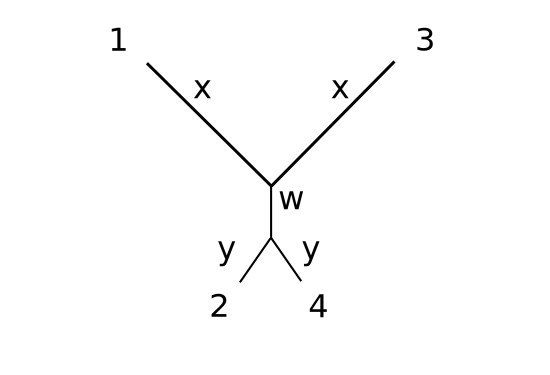
\includegraphics[width=.95\textwidth]{farris_blank}
\caption[short]{Farris topology $\tau_1$}
\end{subfigure}
\begin{subfigure}{.45\linewidth}
\centering
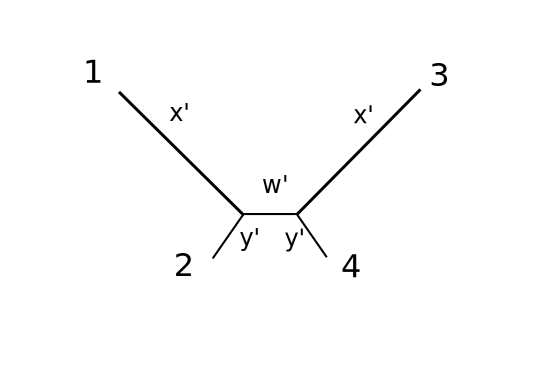
\includegraphics[width=.95\textwidth]{felsenstein_blank}
\caption[short]{Felsenstein topology $\tau_2$}
\end{subfigure}
\caption{Two simple topologies}
\label{fig:farris-fels-top}
\end{figure}

Define the Farris topology $\tau_1$ and the Felsenstein topology $\tau_2$ as in Figure~\ref{fig:farris-fels-top}.
Call $t=\{x,y,w\}$ and $t^*=\{x,y,y\}$, i.e., $t^*$ is the case where the bottom three branches all share the same parameter, the classical construction of this topology.
The branch length parameters are such that the probability of a change in character along the top two branches is $p_x=1-2x$, with corresponding equalities for the other two branches.
Here, $\{p_x,p_y,p_z\}\in[0,1/2]^3$ and $\{x,y,z\}\in[0,1]^3$.

\textbf{Justification for estimand:} It might be worth arguing why this form of the estimand $t$ is necessary.
I think the idea is that for either of these topologies, any maximum obtained will occur where the top two and bottom two branches are equal, though not necessarily the middle branch.
This would be good to show explicitly.

Table~\ref{tab:sitepatprob} contains calculations of site pattern frequencies under these two topologies, calculated using the Hadamard transform approach outlined in 8.6 of Semple and Steel \cite{semplesteel}.
Table~\ref{tab:likelihoods} contains calculations of likelihood values for fixed site patterns and topologies, with the maximum values over ancestral state patterns noted.

\begin{table}
\centering
\begin{tabular}{|l|l|l|}
\multicolumn{3}{c}{Classical}\\
    \hline
$s_j$   &$P(s_j|\tau_1,t^*)$&$P(s_j|\tau_2,t^*)$\\
    \hline
0000&$1+x^2+y^2+4xy^2+x^2y^2$&$1+2xy+2xy^2+x^2y+y^3+x^2y^2$\\
0001&$1+x^2-y^2-x^2y^2$&$1+x^2y-y^3-x^2y^2$\\
0010&$1-x^2+y^2-x^2y^2$&$1-x^2y+y^3-x^2y^2$\\
0100&$1+x^2-y^2-x^2y^2$&$1+x^2y-y^3-x^2y^2$\\
1000&$1-x^2+y^2-x^2y^2$&$1-x^2y+y^3-x^2y^2$\\
0011&$1-x^2-y^2+x^2y^2$&$1+2xy-2xy^2-x^2y-y^3+x^2y^2$\\
0101&$1+x^2+y^2-4xy^2+x^2y^2$&$1-2xy-2xy^2+x^2y+y^3+x^2y^2$\\
1001&$1-x^2-y^2+x^2y^2$&$1-2xy+2xy^2-x^2y-y^3+x^2y^2$\\
    \hline
\multicolumn{3}{c}{Modified}\\
    \hline
$s_j$   &$P(s_j|\tau_1,t)$&$P(s_j|\tau_2,t)$\\
    \hline
0000&$1+x^2+y^2+4xyw+x^2y^2$&$1+2xy+2xyw+x^2w+y^2w+x^2y^2$\\
0001&$1+x^2-y^2-x^2y^2$&$1+x^2w-y^2w-x^2y^2$\\
0010&$1-x^2+y^2-x^2y^2$&$1-x^2w+y^2w-x^2y^2$\\
0100&$1+x^2-y^2-x^2y^2$&$1+x^2w-y^2w-x^2y^2$\\
1000&$1-x^2+y^2-x^2y^2$&$1-x^2w+y^2w-x^2y^2$\\
0011&$1-x^2-y^2+x^2y^2$&$1+2xy-2xyw-x^2w-y^2w+x^2y^2$\\
0101&$1+x^2+y^2-4xyw+x^2y^2$&$1-2xy-2xyw+x^2w+y^2w+x^2y^2$\\
1001&$1-x^2-y^2+x^2y^2$&$1-2xy+2xyw-x^2w-y^2w+x^2y^2$\\
    \hline
\end{tabular}    
\caption{Site pattern probabilities.
All values are multiplied by $1/8$.}
\label{tab:sitepatprob}
\end{table}

\begin{table}
\centering
\begin{tabular}{|l|ll|}
\multicolumn{3}{c}{$P(z_j|s_j,\tau_1,t)$}\\
\hline
& \multicolumn{2}{|c|}{$z_j$}\\
    \hline
$s_j$    &00                              &01\\
    \hline
0000&$(1+x)^2   (1+w)(1+y)^{2*}$          &$(1+x)^2   (1-w)(1-y)^2$\\
0001&$(1+x)^2   (1+w)(1+y)(1-y)^*$        &$(1+x)^2   (1-w)(1+y)(1-y)$\\
0010&$(1+x)^2   (1+w)(1+y)(1-y)^*$        &$(1+x)^2   (1-w)(1+y)(1-y)$\\
0100&$(1+x)(1-x)(1+w)(1+y)^{2*}$          &$(1+x)(1-x)(1-w)(1-y)^2$\\
1000&$(1+x)(1-x)(1+w)(1+y)^{2*}$          &$(1+x)(1-x)(1-w)(1-y)^2$\\
0011&$(1+x)(1-x)(1+w)(1+y)(1-y)^{\dagger}$&$(1+x)(1-x)(1-w)(1+y)(1-y)$\\
0101&$(1+x)^2   (1+w)(1-y)^{2\ddagger}$   &$(1+x)^2   (1-w)(1+y)^{2\ddagger}$\\
1001&$(1+x)(1-x)(1+w)(1+y)(1-y)^{\dagger}$&$(1+x)(1-x)(1-w)(1+y)(1-y)$\\
    \hline
    \hline
&10                           &11\\
    \hline
0000&$(1-x)^2   (1-w)(1+y)^2$     &$(1-x)^2   (1+w)(1-y)^2$\\
0001&$(1-x)^2   (1-w)(1+y)(1-y)$  &$(1-x)^2   (1+w)(1+y)(1-y)$\\
0010&$(1-x)^2   (1-w)(1+y)(1-y)$  &$(1-x)^2   (1+w)(1+y)(1-y)$\\
0100&$(1+x)(1-x)(1-w)(1+y)^2$     &$(1+x)(1-x)(1+w)(1-y)^2$\\
1000&$(1+x)(1-x)(1-w)(1+y)^2$     &$(1+x)(1-x)(1+w)(1-y)^2$\\
0011&$(1+x)(1-x)(1-w)(1+y)(1-y)$  &$(1+x)(1-x)(1+w)(1+y)(1-y)^{\dagger}$\\
0101&$(1-x)^2   (1-w)(1-y)^2$     &$(1-x)^2   (1+w)(1+y)^{2\ddagger}$\\
1001&$(1+x)(1-x)(1-w)(1+y)(1-y)$  &$(1+x)(1-x)(1+w)(1+y)(1-y)^{\dagger}$\\
    \hline
    \multicolumn{3}{c}{$P(z_j|s_j,\tau_2,t)$}\\
\hline
& \multicolumn{2}{|c|}{$z_j$}\\
    \hline
$s_j$    &00                              &01\\
    \hline
0000&$(1+x)^2   (1+w)(1+y)^{2*}$           &$(1+x)(1-x)(1-w)(1+y)(1-y)$\\
0001&$(1+x)^2   (1+w)(1+y)(1-y)^{\ddagger}$&$(1+x)(1-x)(1-w)(1+y)^{2\ddagger}$\\
0010&$(1+x)(1-x)(1+w)(1+y)^{2\ddagger}$    &$(1+x)^2   (1-w)(1+y)(1-y)^{\ddagger}$\\
0100&$(1+x)^2   (1+w)(1+y)(1-y)^{\ddagger}$&$(1+x)(1-x)(1-w)(1-y)^2$\\
1000&$(1+x)(1-x)(1+w)(1+y)^{2\ddagger}$    &$(1-x)^2   (1-w)(1+y)(1-y)$\\
0011&$(1+x)(1-x)(1+w)(1+y)(1-y)^{\ddagger}$&$(1+x)^2   (1-w)(1+y)^{2\ddagger}$\\
0101&$(1+x)^2   (1+w)(1-y)^{2\ddagger}$    &$(1+x)(1-x)(1-w)(1+y)(1-y)^{\ddagger}$\\
1001&$(1+x)(1-x)(1+w)(1+y)(1-y)^{\ddagger}$&$(1-x)^2   (1-w)(1+y)^{2\ddagger}$\\
    \hline
    \hline
&10                           &11\\
    \hline
0000&$(1+x)(1-x)(1-w)(1+y)(1-y)$             &$(1-x)^2   (1+w)(1-y)^2$\\
0001&$(1+x)(1-x)(1-w)(1-y)^2$                &$(1-x)^2   (1+w)(1+y)(1-y)$\\
0010&$(1-x)^2   (1-w)(1+y)(1-y)$             &$(1+x)(1-x)(1+w)(1-y)^2$\\
0100&$(1+x)(1-x)(1-w)(1+y)^{2\ddagger}$      &$(1-x)^2   (1+w)(1+y)(1-y)$\\
1000&$(1+x)^2   (1-w)(1+y)(1-y)^{\ddagger}$  &$(1+x)(1-x)(1+w)(1-y)^2$\\
0011&$(1-x)^2   (1-w)(1-y)^2$                &$(1+x)(1-x)(1+w)(1+y)(1-y)^{\ddagger}$\\
0101&$(1+x)(1-x)(1-w)(1+y)(1-y)^{\ddagger}$  &$(1-x)^2   (1+w)(1+y)^{2\ddagger}$\\
1001&$(1+x)^2   (1-w)(1-y)^{2\ddagger}$      &$(1+x)(1-x)(1+w)(1+y)(1-y)^{\ddagger}$\\
\hline
\end{tabular}    
\caption{Likelihood calculations for all site patterns and internal states of Farris topology.
Maxima determined row-wise (i.e., by site pattern).
All values multiplied by $1/32$.
Key: $^*$ unique maximum value corresponding to unique internal state; $^\dagger$ unique maximum value corresponding to multiple internal states; $^\ddagger$ multiple maximum values corresponding to multiple internal states.}
\label{tab:likelihoods}
\end{table}

\subsection{Bounding the likelihoods}

To simplify matters, we will first focus on bounding the the terms with the generating probabilities as they are more complicated.
Assume $\tau^*=\tau_1$ and $t^*=\{x,y,y\}$ so that
\begin{align}
\label{eq:information}
H_{\tau'}(x, y;x', y', w') &= \sum_{j} P(s_j | \tau_1, \{x,y,y\}) \cdot \log P(s_j | \tau', \{x',y',w'\}) \nonumber \\ 
&:= \sum_{j} p(s_j) \cdot \log P(s_j | \tau', \{x',y',w'\}).
\end{align}
By Gibbs inequality,
$$
H_{\tau'}(x, y;x', y', w') \le H_{\tau'}(x, y;x, y, y),
$$
though this bound can be made tighter.

\textbf{Show}: where these simplifications come about.
It's just adding/subtracting $\log$ terms, but could be good to walk through.

In our simplifications we will make use of the constants
$$
a = p(0100) + p(1000) + p(0011) + p(1001) = (4-2x^2-2y^2)/8,
$$
$$
b = p(1000) + p(0010) + p(0011) + p(1001) = (4-2x^2-2y^2)/8,
$$
$$
c = p(0001) + p(0010) + p(0100) + p(1000) = (4-4x^2y^2)/8
$$
and
$$
d = p(0101) + p(1001) = (2-4xy^2+2x^2y^2)/8
$$
with corresponding bounds
$$
0 \le a,b,c \le \frac{1}{2}
$$
and
$$
0 \le d \le \frac{1}{4}.
$$

Our key approach will be to decompose the likelihood as
\begin{equation}
\label{eq:partial-likelihood}
L^{(i)}(x', y', w') = H_{\tau'}(x,y;x',y',w') + L^{p,(i)}(x',y',w')
\end{equation}
where the first term is \eqref{eq:information} and the second term will be a weighted sum of the $\log$s of values from Table~\ref{tab:likelihoods}, the superscript indicating which choices for ancestral state likelihood values we choose.
Define
$$
\{\hat{x}, \hat{y}, \hat{w}, \hat{i}\} = \arg\max_{\{x,y,w,i\}} \ L^{p,(i)}(x,y,w).
$$
We have upper and lower bounds for \eqref{eq:partial-likelihood} in the form
$$
H_{\tau'}(x,y; \hat{x}, \hat{y}, \hat{w}) + L^{p,(\hat{i})}(\hat{x}, \hat{y}, \hat{w}) \le \max_{x,y,w} \ L^{(i)}(x,y,w) \le H(x,y;x,y,y) + L^{p,(\hat{i})}(\hat{x}, \hat{y}, \hat{w}).
$$

\textbf{Argument for lower bound}: This makes intuitive sense, though may be difficult to show in general.
Can we not just say $\max_u f(u) + g(u)$ is greater than $f(u') + g(u')$ for any $u'$ that doesn't maximize $f(u) + g(u)$ just by definition?
There could be multiple maxima, but that's why we have greater than or equal to.
I think the only thing we'd need to show is that a maximum exists, but since $\{x,y,w\}$ are supported on a closed set this is certainly true.
I must be missing something.

\textbf{Argument for upper bound}: I think this is true mostly because $\max_u f(u) + g(u)$ should be less than $\max_u f(u) + \max_u g(u)$ by some triangle inequality argument.
If we were to actually maximize the full likelihood, we should get something smaller than maximizing some form of it that we consider by looking at the parts separately.
For a fixed $\{x^*, y^*\}$ we can calculate this upper bound directly---can we obtain it as a useful-looking function of these parameters in the general case?

\subsubsection{A simplified Farris likelihood}

The likelihood for the Farris topology is less complicated than that of the Felsenstein since only one site pattern has an ambiguous likelihood---all site patterns except \texttt{0101} have a fixed value for their likelihood when taking the maximum.
To fix this value, we will consider an upper bound on the partial likelihood by setting the value for site pattern 0011 to $(1+x)^2(1+w)(1+y)^2$.
Here the partial likelihood $L_{fa}^{p,(i)}(x,y,w)$ takes the form:
$$
L_{fa}^{p} = (2-a)\log(1+x)+a\log(1-x)+(2-b)\log(1+y)+b\log(1-y)+\log(1+w),
$$
and this has a maximum
$$
\hat{L}_{fa}^{p} = (2-a)\log(2-a)+a\log(a)+(2-b)\log(2-b)+b\log(b)+\log(2).
$$

\subsubsection{A simplified Felsenstein likelihood}

We construct similar bounds on the Felsenstein likelihood, though to make matters simpler we replace all $(1+y)$ terms in Table~\ref{tab:likelihoods} with $(1-y)$ to obtain a lower bound.
Unlike the Farris partial likelihood, the likelihood in this case has one of six forms:
$$
L_{fe}^{(1)} = 2\log(1+x)+(2-c-2d)\log(1+y)+(c+2d)\log(1-y)+\log(1-w),
$$
$$
L_{fe}^{(2)} = (2-c-2d)\log(1+x)+(c+2d)\log(1-x)+2\log(1+y)+\log(1-w),
$$
$$
L_{fe}^{(3)} = (2-2d)\log(1+x)+2d\log(1-x)+(2-c)\log(1+y)+c\log(1-y)+\log(1-w),
$$
$$
L_{fe}^{(4)} = (2-c)\log(1+x)+c\log(1-x)+(2-2d)\log(1+y)+2d\log(1-y)+\log(1-w),
$$
$$
L_{fe}^{(5)} = (2-d)\log(1+x)+d\log(1-x)+(2-c-d)\log(1+y)+(c+d)\log(1-y)+\log(1-w)
$$
and
$$
L_{fe}^{(6)} = (2-c-d)\log(1+x)+(c+d)\log(1-x)+(2-d)\log(1+y)+d\log(1-y)+\log(1-w)
$$
with maxima
$$
\hat{L}_{fe}^{(1)} = \hat{L}_{fe}^{(2)} = 2\log(2)+(2-c-2d)\log(2-c-2d)+(c+2d)\log(c+2d)
$$
$$
\hat{L}_{fe}^{(3)} = \hat{L}_{fe}^{(4)} = (2-2d)\log(2-2d)+2d\log(2d)+(2-c)\log(2-c)+c\log(c)
$$
and
$$
\hat{L}_{fe}^{(5)} = \hat{L}_{fe}^{(6)} = (2-d)\log(2-d)+d\log(d)+(2-c-d)\log(2-c-d)+(c+d)\log(c+d).
$$

\textbf{TODO}: cases for $\{x, y\}$ where each of the above is the corresponding maximum.
I think the first is always greater than or equal to the other two, but I haven't been able to show it yet.
It may take a little information theory--fu, or just standard application of the bounds in the introduction to this section.

\subsubsection{Example}

Set $\{x, y\} = \{0.25, 0.25\}$.
For a Farris zone generating topology, we have
$$
a = b = 0.46875
$$
resulting in
$$
\hat{L}_{fa}^{p}(\hat{x}, \hat{y}, \hat{w}) \approx -2.17803560694
$$
and
$$
H_{fa}(x,y;x,y,y) \approx -2.07509999739.
$$
Computing the upper bound yields
$$
\max_{x,y,w} \ L_{fa}(x,y,w) \le -4.25313560433
$$
and it remains to show that 
$$
\max_{x,y,w} \ L_{fe}(x,y,w) \ge -4.25313560433
$$

For the same generating parameters,
$$
c = 0.498046875, \ d = 0.2431640625,
$$
resulting in
$$
\hat{L}_{fe}(\hat{x}, \hat{y}, \hat{w}) \approx -2.07919739112
$$
Calculating shows%
    %
    \footnote{It's not a typo that $\hat{L}_{fe}$ and $H_{fe}(x,y; \hat{x}, \hat{y}, \hat{w})$ are the same---at least not in the code.
        I should try to show why this is the case.
        }
    %
$$
H_{fe}(x,y; \hat{x}, \hat{y}, \hat{w}) \approx -2.07919739112
$$
and
$$
\max_{x,y,w} \ L_{fe}(x,y,w) \ge -4.15839478224 > -4.25313560433 \ge \max_{x,y,w} \ L_{fa}(x,y,w)
$$
where site patterns are generated from the Farris zone topology.
Confirming, run \texttt{python}'s numerical optimization solver for $\{.25, .25\}$.
Since we are computing a constrained maximization, we can find a global maximum using basin hopping, and doing so yields
$$
\max_{x,y,w} \ L_{fa}(x,y,w) \approx -4.5101771294218045
$$
and
$$
\max_{x,y,w} \ L_{fe}(x,y,w) \approx -4.1544859851260281.
$$
Woohoo!

\subsubsection{General example}

We want to find values for $\{x,y\}$ where
$$
H_{fe}(x,y; 1, 0, 1-c-2d) + \hat{L}_{fe}(c,d) \ge H_{fa}(x,y; x, y, y) + \hat{L}_{fa}(a,b).
$$
We can cheat a bit and plot the values at which this is true.
This may give us some insight into what form these regions of inconsistency take---see Fig.~\ref{fig:inconsistency-farris}.

\begin{figure}
\centering
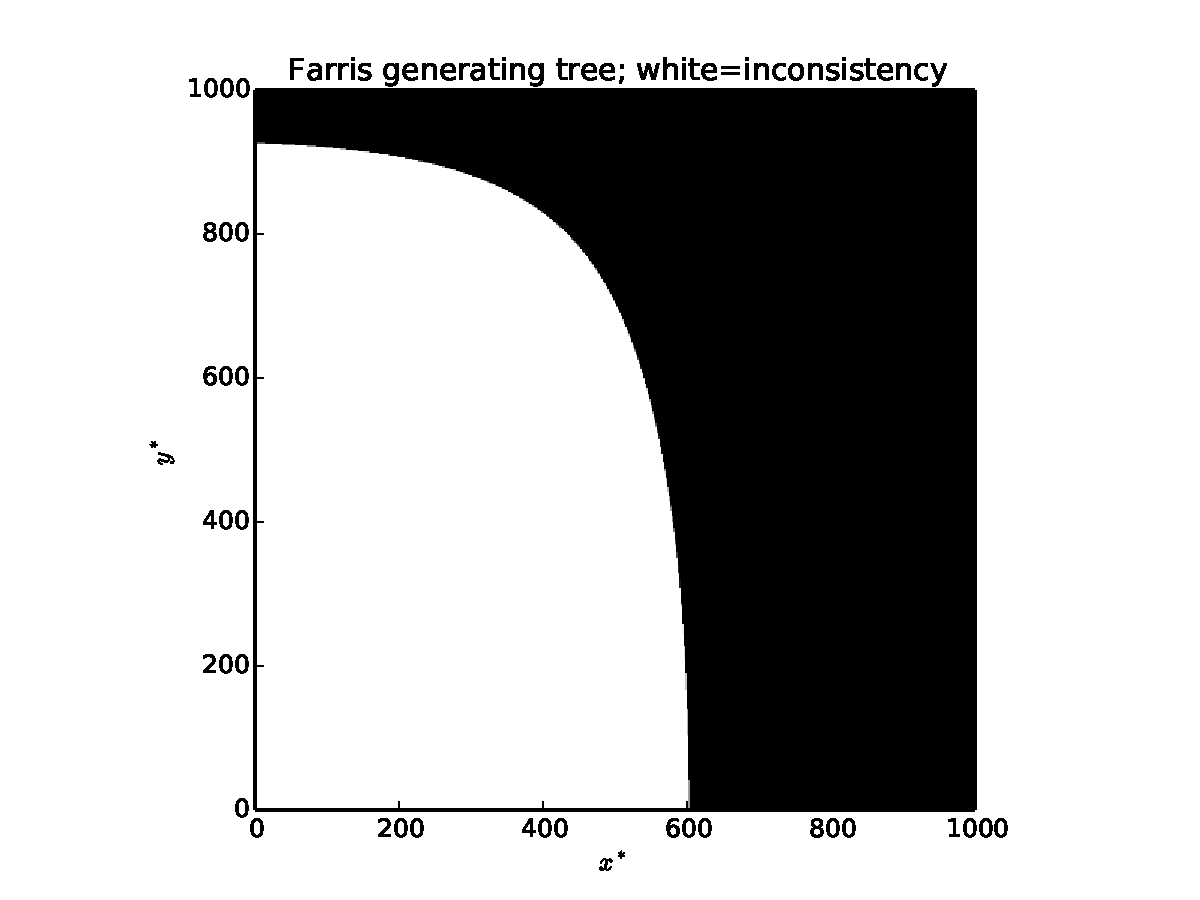
\includegraphics[width=.9\textwidth]{ineqs-max-far-gen}
\caption{Regions of inconsistency}
\label{fig:inconsistency-farris}
\end{figure}

\bibliographystyle{plain}
\bibliography{sample}

\end{document}
